\chapter{Event Generation, Simulation and Reconstruction}
\label{chap:Reconstruction}
\begin{comment}
\section{Computing and Software Tools}

\subsection{Analysis Software}

\subsection{Monte Carlo Event Generators and Simulation Software}

\section{Reconstruction of Jets} 
A head-on collision between two protons taking place at very high energies can be visualized as an interaction between their constituent quarks and gluons. In a hard scattering process i.e. where the momentum transfer is large, the scattered partons fragment and hadronize into highly collimated bunches of particles. The showers of particles get deposited in the calorimeters in the form of conical structures called ``jets''. The clustering of the particles is performed by using jet algorithms, discussed in Sec.~\ref{sec:jet_algos}, and taking partons, stable particles or reconstructed particle candidates as inputs. The different levels at which the jets are formed are parton level, particle level and reconstructed level, as illustrated in Fig.~\ref{fig:jets}. %The charged hadrons ($\sim$60\%), photons ($\sim$30\%) and neutral hadrons ($\sim$10\%) constitute the jets. The photons are reconstructed from ECAL. The charged hadrons are reconstructed from tracker and HCAL and the neutral ones are reconstructed from both ECAL and HCAL.
\begin{figure}[!h]
\begin{center}
\vspace*{3mm} 
\hspace*{-5mm}
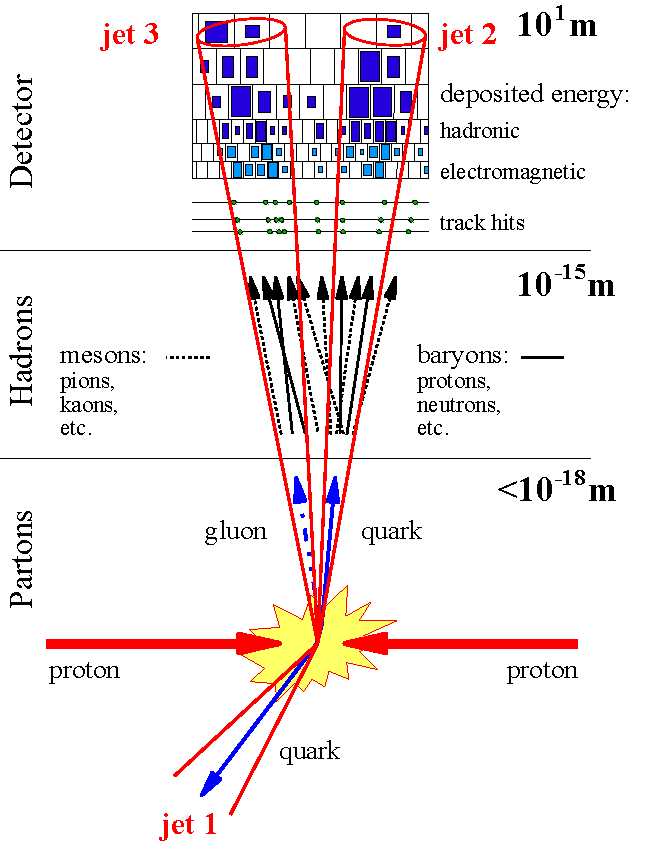
\includegraphics[scale = 0.95]{/home/anter/Desktop/Thesis/Figures/jet_levels_en.pdf}\\
\vspace*{4mm}
\caption{In a proton-proton collision, the hard scattered quarks and gluons fragment and hadronize to produce the showers of partons, hadrons, or detector measurements which are clustered into parton jets, particle jets and reconstructed jets, respectively. Taken from \cite{Schorner-Sadenius:2015cga}.}
\label{fig:jets}
\end{center}
\end{figure}
In the CMS detector, jets are the localized deposits of energy in the calorimeter cells along with the large number of tracks in the direction of the deposited energy. Depending on the type of input to the jet algorithm, the different reconstruction techniques are available. The jets reconstructed using the energy clusters deposited in the calorimeters are called Calorimeter jets (CaloJets) and the ones clustered by taking particle flow candidates as an input give Particle Flow jets (PFJets). 

The analysis presented in this thesis studies the jets clustered using the anti-\kt algorithm with a jet size parameter of R = 0.7 and particle flow candidates. All the particles are reconstructed and identified using a particle-flow (PF) algorithm, discussed in details in next section.

\subsection{Particle Flow Algorithm}
To identify and reconstruct the particles, the CMS employs the event reconstruction technique, Particle Flow (PF) algorithm \cite{CMS:2009nxa, CMS:2010byl}, which combines the information from the individual subdetectors. All the stable particles : electrons, muons, photons, charged and neutral hadrons are reconstructed as well as missing transverse energy (\ETmiss) is determined using PF algorithm. \ETmiss is given by the negative vector sum of transverse momemta \pt of all the isolated stable particles reconstructed in an event i.e. \ETmiss = $-\sum\limits_{\rm i}^{}\overrightarrow{p_{\rm T,i}}$. %= $-\sum\limits_{\rm i\epsilon PF_{particles}}^{}\overrightarrow{p_{\rm T,i}}$
The transverse momenta of final state stable particles or energies of the calorimeter towers are the inputs to PF algorithm. The additional information of the tracking system enhances the reconstruction performance. The PF algorithm uses the information from the tracks and vertices, hits in the tracking detectors, the energy deposits in ECAL and HCAL as well as the tracks in the muon system. The Combinatorial Track Finder (CTF) algorithm \cite{Adam:2005cg} is used to identify the tracks. Based on these tracks, the primary vertices in an event are identified. 





The electromagnetic and hadronic calorimeters are divided into a grid of cells based on the detector granularity to identify calorimeter cluster seeds. If there are seeds with an energy exceeding a certain threshold, they are used in an iterative merging algorithm to form Particle Flow clusters. The different elements of the detector information are then linked together into Particle Flow building blocks based on the geometry and χ 2 fits. At first, muons, which can be well identified using the tracks in the muon detector, are reconstructed using the building blocks connected to the muon system. Blocks connecting the inner tracking system with the ECAL clusters are used to identify electrons. Similarly, charged hadrons are identified using links between the tracking system and the remaining calorimeter clusters. Only neutral objects which leave no traces in the tracking system, remain. ECAL clusters are interpreted as photon candidates, while the remaining HCAL clusters are assumed to be deposits of neutral hadrons. To avoid any kind of double-counting of energy, all Particle Flow building blocks of successfully reconstructed particle candidates are removed and the energy of the calorimeter clusters is recalculated. Finally, a set of so-called Particle Flow candidates is yielded. They consist of well identified particles, which profit from the improved resolution gained by the inclusion of tracking information. This collection of particles is then used to reconstruct the jets and further physical objects.
\end{comment}
